% Options for packages loaded elsewhere
\PassOptionsToPackage{unicode}{hyperref}
\PassOptionsToPackage{hyphens}{url}
%
\documentclass[
]{article}
\usepackage{amsmath,amssymb}
\usepackage{lmodern}
\usepackage{iftex}
\ifPDFTeX
  \usepackage[T1]{fontenc}
  \usepackage[utf8]{inputenc}
  \usepackage{textcomp} % provide euro and other symbols
\else % if luatex or xetex
  \usepackage{unicode-math}
  \defaultfontfeatures{Scale=MatchLowercase}
  \defaultfontfeatures[\rmfamily]{Ligatures=TeX,Scale=1}
\fi
% Use upquote if available, for straight quotes in verbatim environments
\IfFileExists{upquote.sty}{\usepackage{upquote}}{}
\IfFileExists{microtype.sty}{% use microtype if available
  \usepackage[]{microtype}
  \UseMicrotypeSet[protrusion]{basicmath} % disable protrusion for tt fonts
}{}
\makeatletter
\@ifundefined{KOMAClassName}{% if non-KOMA class
  \IfFileExists{parskip.sty}{%
    \usepackage{parskip}
  }{% else
    \setlength{\parindent}{0pt}
    \setlength{\parskip}{6pt plus 2pt minus 1pt}}
}{% if KOMA class
  \KOMAoptions{parskip=half}}
\makeatother
\usepackage{xcolor}
\usepackage[margin=1in]{geometry}
\usepackage{graphicx}
\makeatletter
\def\maxwidth{\ifdim\Gin@nat@width>\linewidth\linewidth\else\Gin@nat@width\fi}
\def\maxheight{\ifdim\Gin@nat@height>\textheight\textheight\else\Gin@nat@height\fi}
\makeatother
% Scale images if necessary, so that they will not overflow the page
% margins by default, and it is still possible to overwrite the defaults
% using explicit options in \includegraphics[width, height, ...]{}
\setkeys{Gin}{width=\maxwidth,height=\maxheight,keepaspectratio}
% Set default figure placement to htbp
\makeatletter
\def\fps@figure{htbp}
\makeatother
\setlength{\emergencystretch}{3em} % prevent overfull lines
\providecommand{\tightlist}{%
  \setlength{\itemsep}{0pt}\setlength{\parskip}{0pt}}
\setcounter{secnumdepth}{-\maxdimen} % remove section numbering
\ifLuaTeX
  \usepackage{selnolig}  % disable illegal ligatures
\fi
\IfFileExists{bookmark.sty}{\usepackage{bookmark}}{\usepackage{hyperref}}
\IfFileExists{xurl.sty}{\usepackage{xurl}}{} % add URL line breaks if available
\urlstyle{same} % disable monospaced font for URLs
\hypersetup{
  pdftitle={Predicting Natural Gas Demand in Germany},
  hidelinks,
  pdfcreator={LaTeX via pandoc}}

\title{Predicting Natural Gas Demand in Germany}
\author{true \and true \and true}
\date{2022-12-08}

\begin{document}
\maketitle

{
\setcounter{tocdepth}{2}
\tableofcontents
}
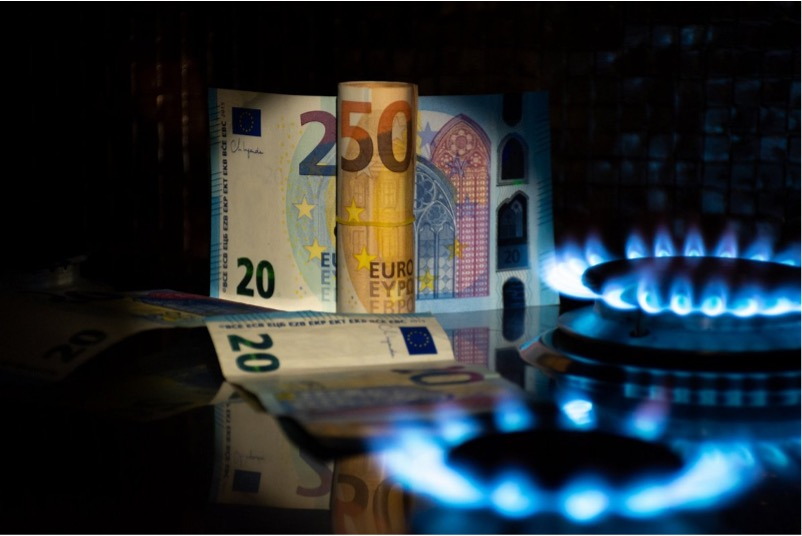
\includegraphics[width=1\linewidth]{figures/Gas1}

\hypertarget{outline}{%
\subsection{Outline}\label{outline}}

\begin{itemize}
\tightlist
\item
  Predicting gas demand is one of the most crucial tasks for the German
  government
\item
  Modelling gas demand is highly complex given its dependence on various
  Supply-side factors (heating vs electricity; industrial vs
  residential)
\item
  Many of these factors are inter-dependent; for e.g.~gas prices,
  exports, GDP
\item
  Demand side factors such as 'responsible demand usage' further
  influence gas demand
\item
  In the past academic literature on modelling gas demand has been
  mostly reliant upon seasonality and less responsive to these immediate
  Demand and Supply (D-S) side shocks
\item
  We use a combination of Auto Regressive and Random Forest models to
  capture both long term seasonal as well as short term D-S shocks
\end{itemize}

\hypertarget{introduction-background}{%
\subsection{Introduction / Background}\label{introduction-background}}

The Russia-Ukraine war has lead Europe towards the largest energy crisis
since the oil price shock of 1973. Since mid-2021, natural gas prices
have been on a steep rise, with average wholesale prices at the TTF spot
market well above 100 C/MWh between October 2021 and mid-2022 and prices
of around 240 C/MWh in August. This is about ten times higher than the
long-term pre-Covid price levels of 15--20 C/MWh (Ruhnau et al 2022).

Germany is an interesting case study to explore gas demand, as it is the
largest export market for Russian natural gas. Furthermore, natural gas
plays an essential role in Germany's industrial production as well as
space heating. Reductions in Germany can therefore make a substantial
contribution to solving the crisis at a European level. In order to
effectively reduce the amount of gas demanded, it is crucial to have
some foresight into how much gas will be demanded in the future. To that
end, we will aim to predict daily German gas demand by implementing a
variety of Machine Learning models.

\hypertarget{our-approach}{%
\subsection{Our Approach}\label{our-approach}}

Existing research on energy demand prediction mostly makes use of
classical, econometric autoregressive modelling techniqes and only
sparsely incorporate machine learning methods. Much of the literature
concerning the forecast of gas demand applies Time Series (TS) models
(Zhang, 2020).

We make use of a combination of models and by splitting the test-train
data both randomly and chronologically, we assess their strengths. Below
is a quick summary of these:

\begin{enumerate}
\def\labelenumi{\roman{enumi}.}
\item
  Static models that use a variety of predictive variables including
  weather and economic factors. They also function well as benchmark
  models for comparative purposes
\item
  Autoregressive Integrated Moving (ARIMA) models used to convert a
  non-stationary time series into a stationary one, and then predict
  future values from historical data. These models are good short term
  predictors but poor long term forecasting models i.e.~not ideal for
  identifying unprecedented events.
\item
  Auto Regressive (AR) models are a special case of the more general
  ARIMA models of time series, which have a more complicated stochastic
  structure. It specifies that the output variable depends linearly on
  its own previous values and on a stochastic term.
\item
  Seasonal Autoregressive Integrated Moving Average with exogenous
  factors, or SARIMAX, is an extension of the ARIMA class of models.
  Unlike the ARIMA, it can capture seasonality in the model. This
  enables it to provide qualified annual forecasting for demand of gas.
\item
  Stochastic Gradient Descent (SGD) because of their ability to cope
  with large-scale datasets;
\item
  Random Forests (RF) as an ensemble learning method, because it works
  particularly well when having a large number of correlated predictors.
\item
  Combinations of the above
\end{enumerate}

\hypertarget{data-we-used}{%
\subsection{Data we used}\label{data-we-used}}

We compiled a dataset consisting of 1833 daily observations (roughly 5
years) and 510 predictor variables, including transformations. For all
variables, including date transformations, we add ln, square and
elasticity transformations. Additionally, a 7-day lagged copy of all
variables except date features is added. Our key variables were; Daily
national gas demand, Gas prices, Weather data from various cities within
Germany, Co2 Prices, Electricity Prices, DAX and Quarterly GDP.

\hypertarget{key-findings}{%
\subsection{Key Findings}\label{key-findings}}

\emph{Our key findings are summarized below:}

\begin{itemize}
\tightlist
\item
  As demand can be predicted using weather and economic data; the
  proof-of-concept Linear SGD Model with chronological split performs
  with R2 = 0.9039,
\item
  Gas demand is strongly autocorrelated; when building simple AR models,
  the best model is a Random Forest with random split, performing with
  R2 = 0.9446,
\item
  Seasonal patterns matter; when extending to SAR models, the best model
  is a Random Forest with random split, performing with R2 = 0.9644,
\item
  Machine Learning models win over classical econometrical models; the
  SARIMAX model with chronological split performs with R2 = 0.8150,
  confirming that there is strong autocorrelation in place in any case.
\item
  The best model is a Random Forest with random split, performing with
  R2 = 0.9794. When comparing RMSE values, it outperforms the
  preliminary model.
\end{itemize}

\emph{More generally, we find:}

\begin{itemize}
\tightlist
\item
  In almost all model configurations, Random Forest models outperform
  Linear SGD models,
\item
  Our combination strategy works: pairing autoregressive and machine
  learning modeling approaches increases the predictive strength. The
  SAR ML models with full variable configuration do the trick and are
  able to catch the underlying principles of gas demand.
\end{itemize}

Below you can find a visual representation of the fit of some of the
models we used.

\begin{figure}
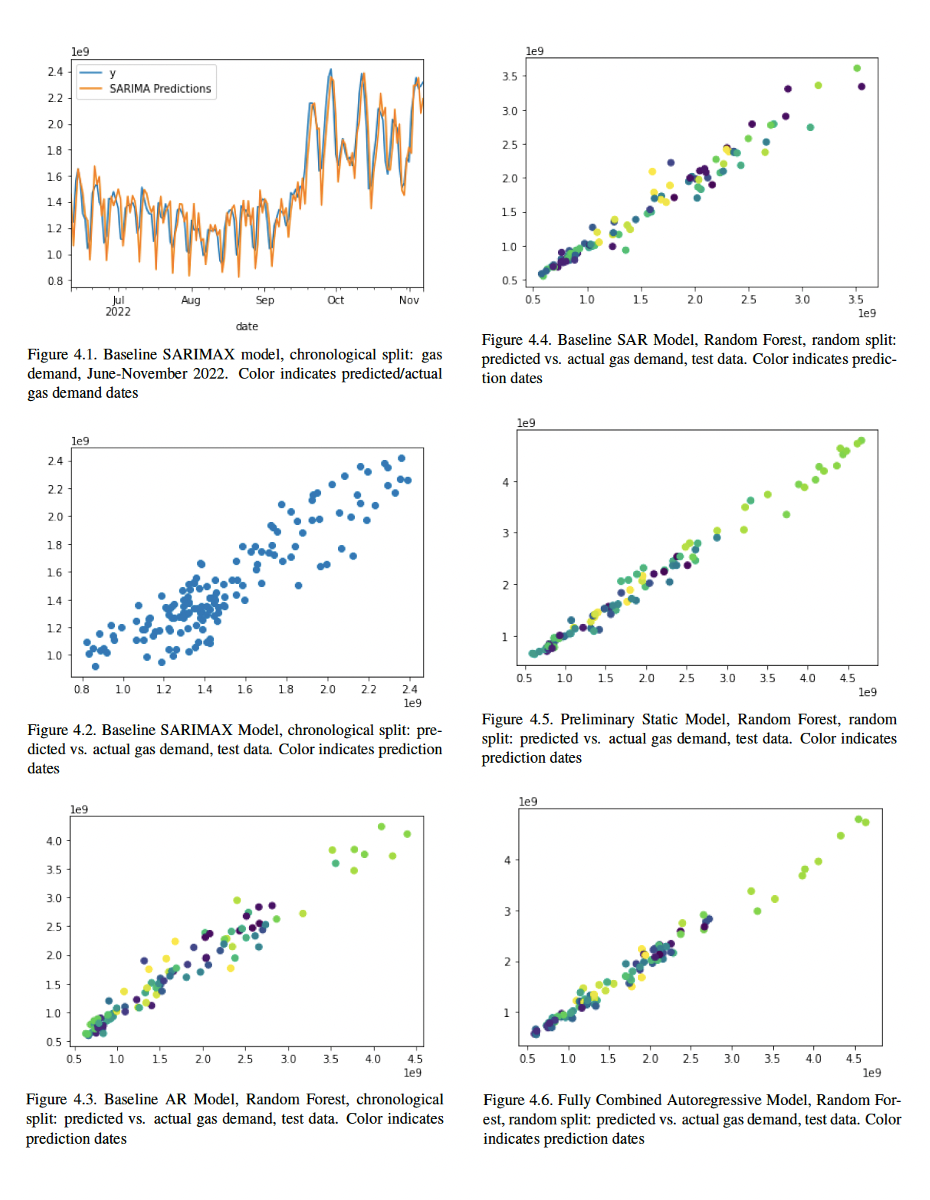
\includegraphics[width=1\linewidth]{figures/Gas2} \caption{Snapshot from our Research paper on the various models used}\label{fig:unnamed-chunk-2}
\end{figure}

\end{document}
